\section{能量估计}
\label{sec:wave-energy}

前面的计算反复出现同一个量：弦的动能加弹性能。不写出解，只对方程乘$\partial_tu$再积分，能得到什么？这样得到的结论不依赖一维公式，也不依赖模式展开，在一般区域上同样成立。

\paragraph{动能和弹性能}
线密度为$\rho$的弦，一小段的动能是$\frac12\rho(\partial_tu)^{2}\,\mathrm{d}x$。弹性能等于张力乘以伸长量，小斜率时一小段的伸长是$\sqrt{1+(\partial_xu)^{2}}\,\mathrm{d}x-\mathrm{d}x\approx\frac12(\partial_xu)^{2}\,\mathrm{d}x$，所以弹性能是$\frac12\kappa(\partial_xu)^{2}\,\mathrm{d}x$。除以$\rho$并推广到$\Omega\subset\mathbb{R}^{d}$，定义\term{动能}（kinetic energy）和\term{弹性能}（elastic energy）之和
\begin{equation}
 E(t)=\frac12\int_\Omega\bigl[(\partial_tu)^{2}+c^{2}\lVert\nabla u\rVert_2^{2}\bigr]\,\mathrm{d}\bm{x}.
 \label{eq:wave-energy}
\end{equation}

\begin{theorem}[能量恒等式]
\label{thm:wave-energy-identity}
设$\Omega\subset\mathbb{R}^{d}$有界，边界分片光滑，$u\in C^{2}(\overline{\Omega}\times[0,T])$满足$\partial_t^{2}u-c^{2}\Delta u=f$。则
\begin{equation}
 E'(t)=\int_\Omega f\,\partial_tu\,\mathrm{d}\bm{x}+c^{2}\int_{\partial\Omega}\partial_tu\,\partial_{\bm{n}}u\,\mathrm{d}S .
 \label{eq:wave-energy-identity}
\end{equation}
特别地，若$f\equiv0$，且边界每一处或者$\partial_tu=0$，或者$\partial_{\bm{n}}u=0$，则$E(t)$为常数。
\end{theorem}

\begin{proof}
积分号下对$t$求导，得到
\[
 E'(t)=\int_\Omega\bigl[\partial_tu\,\partial_t^{2}u+c^{2}\nabla u\cdot\nabla\partial_tu\bigr]\,\mathrm{d}\bm{x}.
\]

第二项用散度定理移走梯度，散度定理的条件和形式可参考\BookChapterRef{chap:integral-theorems}{卷二第27章“积分定理”}：
\[
 \int_\Omega\nabla u\cdot\nabla\partial_tu\,\mathrm{d}\bm{x}=\int_{\partial\Omega}\partial_tu\,\partial_{\bm{n}}u\,\mathrm{d}S-\int_\Omega\partial_tu\,\Delta u\,\mathrm{d}\bm{x}.
\]

代回去，体积分合并成$\int_\Omega\partial_tu(\partial_t^{2}u-c^{2}\Delta u)\,\mathrm{d}\bm{x}$，由方程等于$\int_\Omega f\partial_tu\,\mathrm{d}\bm{x}$。这就是式~\eqref{eq:wave-energy-identity}。无源且边界项为零时，$E'=0$。
\end{proof}

式~\eqref{eq:wave-energy-identity}是能量账：右端第一项是外力的功率，第二项是边界的功率，它正是式~\eqref{eq:wave-end-power}除以$\rho$。固定端、自由端以及给定不随时间变化的位移（此时$\partial_tu=0$）都不进出能量。

\paragraph{和热方程对比}
第~\ref{chap:diffusion-equations}章对热方程也做了能量估计，那里在同样的边界条件下乘的是$u$，得到的是
\[
 \frac{\mathrm{d}}{\mathrm{d}t}\,\frac12\int_\Omega u^{2}\,\mathrm{d}\bm{x}=-\int_\Omega\lVert\nabla u\rVert_2^{2}\,\mathrm{d}\bm{x}\leq0 .
\]
区别在于热方程的能量只含$u$，并且被梯度持续消耗；波动方程的能量同时含$\partial_tu$和$\nabla u$，两部分互相转换，总量不变。这也和两个方程的时间方向性相合：波动方程把$t$换成$-t$仍是波动方程，能量守恒在两个时间方向都成立；热方程只能向前。

\paragraph{手算一个能量账}
继续用中点拨起的弦，$L=1$，$c=1$。$t=0$时速度为零，$\lvert u_0'\rvert=1$几乎处处成立，所以由式~\eqref{eq:wave-energy}，
\[
 E(0)=\frac12\int_0^{1}1\,\mathrm{d}x=\frac12 .
\]

能量也可以按模式计算。把式~\eqref{eq:wave-series}代入式~\eqref{eq:wave-energy}，由三角函数的正交性，不同模式的交叉项为零，每个模式的能量单独守恒：
\begin{equation}
 E=\frac L4\sum_{n=1}^{\infty}\bigl(\omega_n^{2}a_n^{2}+b_n^{2}\bigr).
 \label{eq:wave-modal-energy}
\end{equation}

代入式~\eqref{eq:wave-pluck-coefficients}。只有奇数$n$的项非零，$\omega_n^{2}a_n^{2}=16/(n^{2}\pi^{2})$，于是
\[
 E=\frac14\sum_{n\ \text{奇}}\frac{16}{n^{2}\pi^{2}}=\frac4{\pi^{2}}\sum_{n\ \text{奇}}\frac1{n^{2}}=\frac4{\pi^{2}}\cdot\frac{\pi^{2}}8=\frac12 .
\]
两种算法一致。这里折线初值只是分段光滑，定理~\ref{thm:wave-energy-identity}不能直接用，但式~\eqref{eq:wave-modal-energy}对$H_0^{1}\times L^{2}$的数据仍然成立。第一项占$4/\pi^{2}\approx0.405$，即总能量的$81\%$；加上$n=3$后达$90\%$，加上$n=5$后达$93\%$。高频模式的系数虽小，乘上$\omega_n^{2}$后对能量的贡献并不小。

\paragraph{能量守恒不等于振幅不变}
能量不变，弦上各点的位移却可以大幅变化。回到实轴上的帐篷形初值，由式~\eqref{eq:wave-tent-solution}，$t=0$时能量全是弹性能：
\[
 E=\frac12\int_{-1}^{1}1\,\mathrm{d}x=1,\qquad \max_{x}\lvert u(x,0)\rvert=1.
\]

$t\geq1$时分成两列互不重叠的波，每列的$\partial_tu$和$\partial_xu$的平方都是$1/4$，在长度为$2$的支集上，动能和弹性能都是$\frac12\cdot\frac14\cdot2$，两列相加得到
\[
 K=\frac12,\qquad V=\frac12,\qquad \max_{x}\lvert u(x,t)\rvert=\frac12.
\]
最大位移减半，总能量不变，只是一半的弹性能变成了动能。

图~\ref{fig:wave-energy-accounting}对比了这几种情形。(a)是拨弦的动能和弹性能相互转换，总和恒为$1/2$。(b)是同一初值下热方程的$\frac12\lVert u\rVert_2^{2}$，单调衰减。(c)是实轴上的帐篷，总能量不变，最大位移却下降。

\begin{BookInlineFigure}
  \centering
  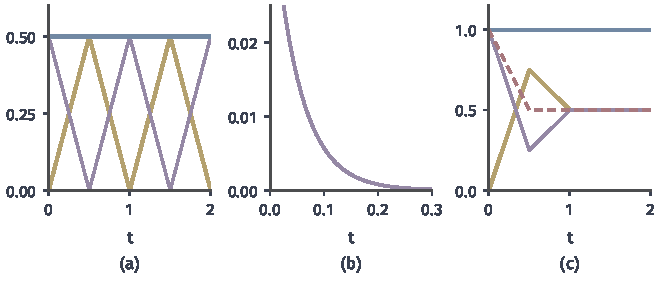
\includegraphics[width=112mm]{figures/06-differential-equations/02-partial-differential-equations/matplotlib/wave-energy-accounting/figure.pdf}
  \caption{能量账。(a)拨弦，$L=1$，$c=1$：黄线是动能，紫线是弹性能，蓝线是两者之和。(b)同一初值在热方程下的$\frac12\lVert u\rVert_2^{2}$（紫），单调下降。(c)实轴上的帐篷：黄、紫、蓝含义同(a)，红色虚线是最大位移，从$1$降到$1/2$，能量却保持为$1$。}
  \label{fig:wave-energy-accounting}
\end{BookInlineFigure}

\paragraph{差解的能量给出唯一性}
能量恒等式最直接的用途是唯一性：设两个解有相同的数据，它们的差的能量从零开始，又不会增加。

\begin{theorem}[唯一性]
\label{thm:wave-uniqueness}
设$\Omega$有界，边界分片光滑。式~\eqref{eq:wave-ibvp}在每一处边界上指定$u$或$\partial_{\bm{n}}u$的条件下，至多有一个$C^{2}(\overline{\Omega}\times[0,T])$解。
\end{theorem}

\begin{proof}
设$u,\tilde{u}$是两个解，$w=u-\tilde{u}$。由线性性，$w$满足无源方程、零初值和齐次的边界条件：在指定$u$的边界上$w=0$，从而$\partial_tw=0$；在指定$\partial_{\bm{n}}u$的边界上$\partial_{\bm{n}}w=0$。定理~\ref{thm:wave-energy-identity}给出$w$的能量为常数，而零初值使它在$t=0$时为零，所以
\[
 \int_\Omega\bigl[(\partial_tw)^{2}+c^{2}\lVert\nabla w\rVert_2^{2}\bigr]\,\mathrm{d}\bm{x}=0,\qquad 0\leq t\leq T.
\]

被积函数连续且非负，所以处处为零，特别地$\partial_tw\equiv0$。于是$w(\bm{x},t)=w(\bm{x},0)=0$。
\end{proof}

边界条件在这里是必需的。在$(0,1)$上取$c=1$，零初值，如果不给边界条件，$u\equiv0$是解，而式~\eqref{eq:wave-boundary-solution}的右行波$g(t-x)$（$g$在$t$很小时为零）也是解：它们的初值相同，差别只来自左端的输入。边界条件正是用来堵住这种能量入口的。

这个证明没有用到解的公式。第~\ref{sec:wave-modes}节的级数解的唯一性由此得到。同样的思路用于有限时间的连续依赖，见下面的增长估计。

\paragraph{外力下的能量增长}
含源项时能量不再守恒，但能估计它增长多快。由式~\eqref{eq:wave-energy-identity}，边界项为零时，Cauchy--Schwarz不等式给出
\[
 E'(t)\leq\lVert f(\cdot,t)\rVert_{L^{2}(\Omega)}\,\lVert\partial_tu(\cdot,t)\rVert_{L^{2}(\Omega)} .
\]

动能不超过总能量，所以$\lVert\partial_tu\rVert_{L^{2}}\leq\sqrt{2E}$，从而
\[
 E'(t)\leq\sqrt2\,\lVert f(\cdot,t)\rVert_{L^{2}(\Omega)}\sqrt{E(t)} .
\]

这种形式的不等式适合对$\sqrt{E}$积分。为了避免$E=0$时除以零，先对$\varepsilon>0$考虑$\sqrt{E+\varepsilon}$，求导后代入上式，得到
\[
 \frac{\mathrm{d}}{\mathrm{d}t}\sqrt{E+\varepsilon}=\frac{E'}{2\sqrt{E+\varepsilon}}\leq\frac1{\sqrt2}\lVert f(\cdot,t)\rVert_{L^{2}(\Omega)} .
\]
积分后令$\varepsilon\to0$，就得到下面的定理。

\begin{theorem}[能量增长估计]
\label{thm:wave-energy-growth}
在定理~\ref{thm:wave-energy-identity}的条件下，设边界项为零。则对$0\leq t\leq T$，
\begin{equation}
 \sqrt{E(t)}\leq\sqrt{E(0)}+\frac1{\sqrt2}\int_0^{t}\lVert f(\cdot,s)\rVert_{L^{2}(\Omega)}\,\mathrm{d}s .
 \label{eq:wave-energy-growth}
\end{equation}
\end{theorem}

用在两组数据的差解上，式~\eqref{eq:wave-energy-growth}给出有限时间内对$(u_0,u_1,f)$的连续依赖，度量是能量范数。

这个估计的增长速度和共振是相合的。继续第~\ref{sec:wave-forced}节的例子，$L=1$，$c=1$，$f=\sin(\pi x)\cos\pi t$。外力的范数和能量分别是
\[
 \lVert f(\cdot,t)\rVert_{L^{2}}=\frac{\lvert\cos\pi t\rvert}{\sqrt2},\qquad E(t)=\frac14\bigl(\dot{a}_1^{2}+\pi^{2}a_1^{2}\bigr),
\]
后者由式~\eqref{eq:wave-modal-energy}对时变系数的同样计算得到。

在$t=12$处，由$a_1=t\sin\pi t/(2\pi)$得$a_1(12)=0$，$\dot{a}_1(12)=6$，所以$\sqrt{E(12)}=3$。式~\eqref{eq:wave-energy-growth}的右端是
\[
 \frac12\int_0^{12}\lvert\cos\pi s\rvert\,\mathrm{d}s=\frac12\cdot12\cdot\frac2\pi=\frac{12}{\pi}\approx3.82 .
\]
上界成立，两者都随$t$线性增长，估计的阶是准确的。如图~\ref{fig:wave-energy-growth}，非共振的$\Omega=2$只让能量有界振荡，这时上界就偏松了：式~\eqref{eq:wave-energy-growth}只用到$\lVert f\rVert_{L^{2}}$，看不到外力和模式频率是否匹配。

\begin{BookInlineFigure}
  \centering
  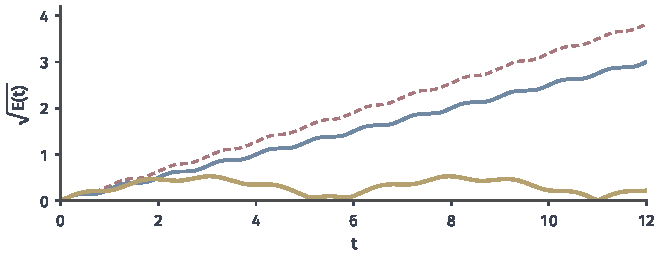
\includegraphics[width=112mm]{figures/06-differential-equations/02-partial-differential-equations/matplotlib/wave-energy-growth/figure.pdf}
  \caption{外力下的$\sqrt{E(t)}$，$L=1$，$c=1$，零初值，$f=\sin(\pi x)\cos\Omega t$。蓝线是共振$\Omega=\pi$，红色虚线是它的上界~\eqref{eq:wave-energy-growth}，两者都线性增长。黄线是非共振$\Omega=2$，能量有界。}
  \label{fig:wave-energy-growth}
\end{BookInlineFigure}
